\chapter{Конформационный анализ производных и гетероаналогов бицикло[3.3.1]нонана (обзор литературы)}

\begin{figure}
\centering
\begin{tabular}{|c|c|c|}
\toprule
\multicolumn{3}{c}{\chemfig{[:-30,1.25]9*6(-1(-[:180]2-[:120]3-[:+60]4-[:0]\phantom{5}?)-8-7-6-5-)}} \\
\multicolumn{3}{c}{\cmpd{Bicycle331} } \\
\midrule
1. & 2. & 3. \\
\chemfig{[:-30]3?-[:-60]2-[:0]1-[:+120]9-[:+60]5-[:+180]4?}\chemfig{[:-30]9*6(-1-8-7-6-5-)} &
\chemfig{[:-30]9*6(-[,,,,dash pattern=on 1pt off 1pt]1(-[:180]2-[:120]3-[:+60]4-[:0]\phantom{5}?)-8-7-6-5-[,,,,dash pattern=on 1pt off 1pt])} & 
\chemfig{[:-30]9*6(-1(-[:180,,,,dash pattern=on 1pt off 1pt]2-[:120]3-[:+60]4-[:0,,,,dash pattern=on 1pt off 1pt]\phantom{5}?)-[,,,,dash pattern=on 1pt off 1pt]8-7-6-[,,,,dash pattern=on 1pt off 1pt]5-)} \\
\bottomrule
\end{tabular}
\vspace{\medskipamount}
    \caption{\label{fig:Decomposition:331} Номенклатура положений и подструктурные декомпозиции системы бицикло[3.3.1]нонана}
\end{figure}

Конформационный анализ сложных систем предполагает их разбиение на~подструктуры с дальнейшим выражением конформации структуры в~целом как суперпозиции конформаций подструктур. Система бицикло[3.3.1]нонана допускает несколько подобных разбиений~(рис.~\ref{fig:Decomposition:331}):

\begin{enumerate}
    \item два 1,3-конденсированных шестичленных цикла: $(1-2-3-4-5-9)$
    и $(5-6-7-8-1-9)$;
    \item восьмичленный цикл с одноатомным мостиком ($9$) между положениями 1 и 5;
    \item три взаимодействующих трёхатомных фрагмента $2-3-4$, $8-7-6$ (так называемые \tqt{крылья}) и $1-9-5$;
\end{enumerate}

Конформация данного бициклического скелета традиционно определяется согласно первому разбиению, т. е., конформациями двух составляющих его шестичленных циклов~(рис.~\ref{fig:System331:379XYZ:Conf}). Для насыщенных производных выделяются конформации \tqt{двойное кресло} (\CC{}), \tqt{кресло-ванна} (\CB{}) и \tqt{двойной ванны} (\BB{}). В случае структурной эквивалентности \tqt{крыльев} наблюдается \emph{конформационное вырождение} "--- формы \CB{} и \BC{} становятся структурно и энергетически неразличимыми. Максимальная пространственная симметрия "--- \(\SymGroup{C}{2v}\) для \CC{} и \BB{}, \(\SymGroup{C}{s}\) для \CB{} и \BC{}.

Для пространственных форм насыщенных шестичленных циклов оптимальной является структура \tqt{кресла}~(\ConfName{К}); форма \tqt{ванна}~(\ConfName{В}) обычно является переходным состоянием в процессе пседовращения между двумя конформерами с \tqt{твист}-структурой~(\ConfName{Т}). Причиной этого признано сильное повышение энергии структур с ординарными связями в заслонённой конформации (так называемое \emph{питцеровское напряжение}). По этой же причине форма \BB{} у~производных бицикло[3.3.1]нонана встречается очень редко (характерна для сильно затруднённых и напряжённых молекул) и обычно наблюдается экспериментально в виде формы «двойного твиста» (\TT{}).

\begin{figure}
\centering
\begin{tabular}{c|c}
\multicolumn{2}{c}{
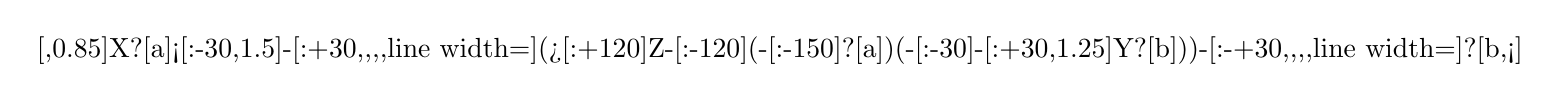
\begin{tikzpicture}
\node(Bicyclo331) at(0,0) {%
\chemfig{[,0.85]X?[a]<[:-30,1.5]-[:+30,,,,line width=\boldbondwidth](>[:+120]Z-[:-120](-[:-150]?[a])(-[:-30]-[:+30,1.25]Y?[b]))-[:-+30,,,,line width=\boldbondwidth]?[b,{<}]} };
\end{tikzpicture}
}
\\
\multicolumn{2}{c}{\BB{}~(\TT{})} \\
\midrule
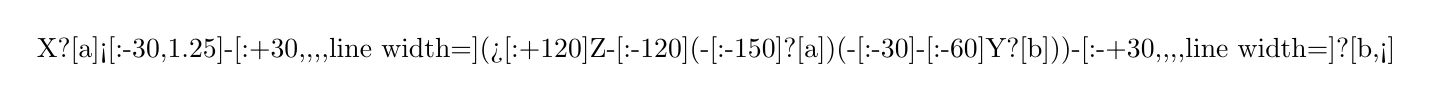
\begin{tikzpicture}
\node(Bicyclo331) at(0,0) {%
\chemfig{X?[a]<[:-30,1.25]-[:+30,,,,line width=\boldbondwidth](>[:+120]Z-[:-120](-[:-150]?[a])(-[:-30]-[:-60]Y?[b]))-[:-+30,,,,line width=\boldbondwidth]?[b,{<}]} };
\end{tikzpicture}
& 
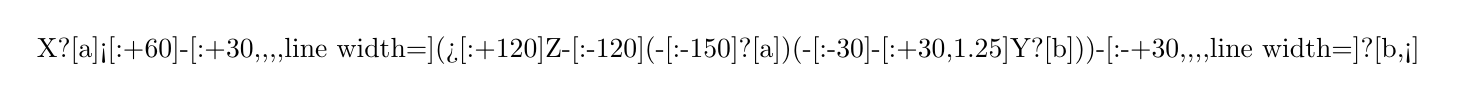
\begin{tikzpicture}
\node(Bicyclo331) at(0,0) {%
\chemfig{X?[a]<[:+60]-[:+30,,,,line width=\boldbondwidth](>[:+120]Z-[:-120](-[:-150]?[a])(-[:-30]-[:+30,1.25]Y?[b]))-[:-+30,,,,line width=\boldbondwidth]?[b,{<}]} 
};
\end{tikzpicture}
\\
\BC{} & \CB{}
\\
\midrule
\multicolumn{2}{c}{%
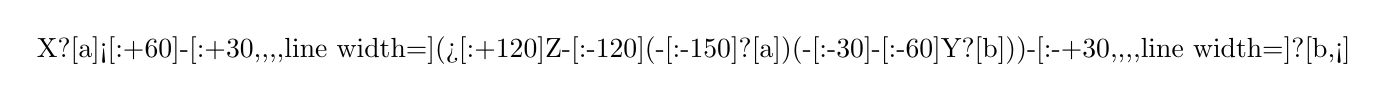
\begin{tikzpicture}
\node(Bicyclo331) at(0,0) {%
\chemfig{X?[a]<[:+60]-[:+30,,,,line width=\boldbondwidth](>[:+120]Z-[:-120](-[:-150]?[a])(-[:-30]-[:-60]Y?[b]))-[:-+30,,,,line width=\boldbondwidth]?[b,{<}]} 
};
\end{tikzpicture}
}
\\
\multicolumn{2}{c}{\CC{}}
\\
\end{tabular}
\caption{\label{fig:System331:379XYZ:Conf} Конформационное поведение несимметричных 3,7.9-замещённых производных бицикло[3.3.1]нонана}
\end{figure}


Торсионные напряжения также являются фактором устойчивости и для формы \CB{}, содержащей подструктуру \tqt{ванны}, в которой, однако, заслонённые конформации связей незначительно отклоняются от идеальной формы \ConfName{В} с эндоциклическими двугранными углами $\tau_{9123}\simeq 0$ и $\tau_{9543}\simeq 0$. Часто эти отклонения симметричны, т. е., $\tau_{9123} = -\tau_{9543}$. Всё это является показателем стереохимической (конформационной) жёсткости формы \tqt{кресла} насыщенного шестичленного цикла. Такая жёсткость образуется из сочетания низкой энергии и высоких собственных частот колебания структуры. Жёсткие конформации одной из подструктур молекулы могут стабилизировать менее энергетически выгодные формы других как термодинамически, так и  кинетически.

Конформация \CC{} состоит из кресловидных шестичленных циклов, почти свободных от питцеровского напряжения. Основным фактором устойчивости для этой конформации оказывается невалентное взаимодействие между положениями 3 и 7. Дисперсионное или электростатическое отталкивание между этими положениями или эндо-заместителями в них приводит к повышению энергии и дестабилизации \CC{} относительно других форм, тогда как притяжение стабилизирует соответствующую структуру.
